Another important quantity to correct for in the unresolved resonance region is capture yield. In these experiments, there are two phenomena at play: first the resonance self shielding, as described in \autoref{sec:resonance-self-shielding}. The second effect is called multiple scattering.

Multiple scattering is an effect which occurs in which a neutron is scattered one or more times before being captured in a sample. As the thickness of the sample increases, the probability of a scattered neutron experiencing a subsequent reaction (that being a capture or additional scattering events) also increases. Therefore, neutrons which undergo scattering events can end up miscounted as captures, artificially increasing the measured yield.
\begin{figure}[H]
    \centering
    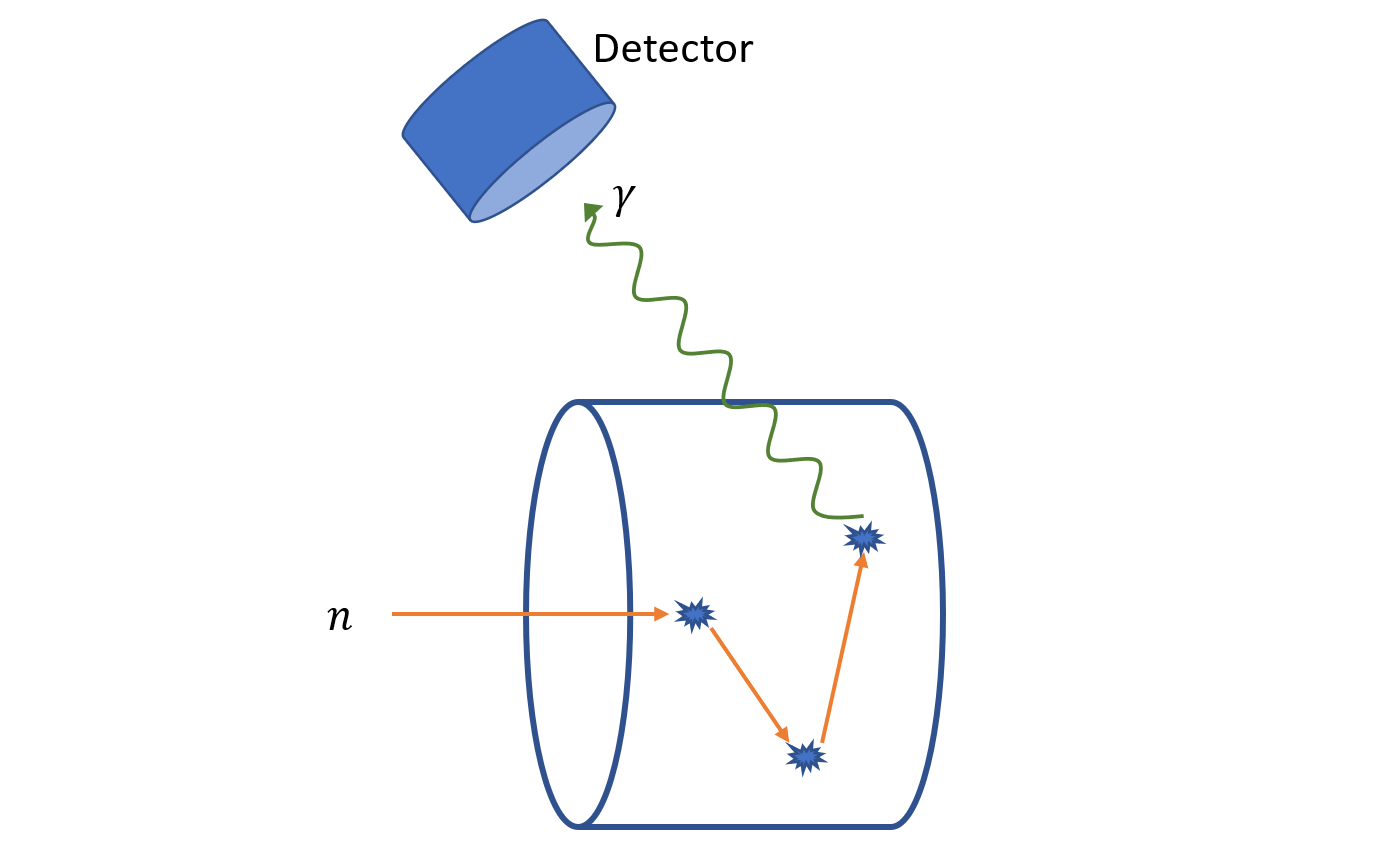
\includegraphics[width=0.75\linewidth]{Figures/multiplescattering.png}
    \caption{Illustration of a neutron undergoing multiple scattering events, and getting miscounted as a capture event.}
    \label{fig:multiple-scattering-example}
\end{figure}
This is illustrated in \autoref{fig:multiple-scattering-example}, in which a neutron scatters twice before being captured.

This correction is made with reference to the thin sample approximation,
\begin{equation}
    \label{eq:thin-sample-approximation}
    \left\langle Y \right\rangle \approx n \left\langle \sigma_\gamma \right\rangle 
\end{equation}
where $\left\langle Y \right\rangle$ is the average yield, $n$ is the sample thickness, and $\left\langle \sigma_\gamma \right\rangle$ is the average capture cross section. The capture correction $C_C$ corrects the thin sample approximation such that
\begin{equation}
    \label{eq:correction-thin-sample-approximation}
    \left\langle Y \right\rangle = n \left\langle \sigma_\gamma \right\rangle C_C
\end{equation}

In order to calculate the correction, a series of Monte Carlo simulations are used to simulate a neutron undergoing a series of capture or scattering events in a cylindrical disc target. The target has a radius $R$, is parallel to the $z$ axis, and with front and rear faces located at $z=0$ and $z=n$, respectively, which are centered at $(x,y)=(0,0)$. A neutron is born at the energy of interest, $E^0$, and is incident on the front face of the target, with the location
\begin{equation}
    \label{eq:incident-neutron-location}
    \overrightarrow{x}^0 = \begin{bmatrix}
        x^0 \\
        y^0 \\
        z^0
    \end{bmatrix} =
    \begin{bmatrix} 
        r_0\cos{\left( \theta_0 \right)} \\
        r_0\sin{\left( \theta_0 \right)} \\
        0
    \end{bmatrix}
\end{equation}
where
\begin{align*}
    r_0 &= R\sqrt{\zeta}, \\
    \theta_0 &= 2\pi\zeta,
\end{align*}
and $\zeta$ is a uniformly distributed random value between 0 and 1. The neutron is also traveling along the $z$-axis, and therefore is born with the direction vector
\begin{equation}
    \label{eq:incident-neutron-location}
    \overrightarrow{\Omega}^0 = \begin{bmatrix}
        \Omega^0_u \\
        \Omega^0_v \\
        \Omega^0_w
    \end{bmatrix} =
    \begin{bmatrix}
        0 \\
        0 \\
        1
    \end{bmatrix}
\end{equation}

Cross sections are sampled at the energy $E^0$ according to the procedure described in \autoref{sec:resonance-sampling}. These values are then used to produce the average cross-sections,
\begin{align}
    \label{eq:average-total-cross-section}
    \overline{ \sigma_{t} }^{0} &= \sum_{j} \sigma_{t,j}^{0} \delta_{j} \\
    \label{eq:average-capture-cross-section}
    \overline{ \sigma_{\gamma} }^{0} &= \sum_{j} \sigma_{\gamma,j}^{0} \delta_{j} \\
    \label{eq:average-scattering-cross-section}
    \overline{ \sigma_{sc} }^{0} &= \sum_{j} \sigma_{sc,j}^{0} \delta_{j}
\end{align}
where $\overline{ \sigma_{t} }$, $\overline{ \sigma_{\gamma} }$, and $\overline{ \sigma_{sc} }$  are the weighted average total, capture, and scattering cross-sections respectively. The $0$ superscript indicates that the cross-sections are taken at the energy $E^{0}$, i.e., before any scattering events have occurred. The terms $\sigma_{j}^0$ and $\delta_{j}$ are the microscopic cross-section and relative abundance of the $j^{th}$ isotope, respectively.

\subsection{Scattering Events}

\subsubsection{Sampling Location}
\label{sec:sampling-location-ms}
The distance to leave the sample is then calculated according to the shortest path to intersect with one of the surfaces in the direction in which the neutron is traveling. For the initial neutron, that is, before any scattering events have occurred, this is just the thickness of the sample $n$. However, for a scattering event this must be solved generally for a neutron that undergone $k$ scattering events. In this case, the neutron would have position vector $\overrightarrow{x}^k$ and direction $\overrightarrow{\Omega}^k$. The quantity that must be determined is the shortest path for it to leave the sample. In the case of a cylindrical target, there are three separate surfaces in which the neutron could escape:
\begin{enumerate}
    \item The front surface at $z=0$,
    \item The rear surface at $z=n$, and
    \item The cylindrical surface at $x^2 + y^2 = R^2$.
\end{enumerate}
Therefore, there are three distances that must be calculated:
\begin{align*}
    d_{front}   &\equiv \text{Distance neutron must travel to intersect with front face} \\
    d_{back}    &\equiv \text{Distance neutron must travel to intersect with back face} \\
    d_{cyl}     &\equiv \text{Distance neutron must travel to intersect with cylindrical surface}
\end{align*}
\begin{figure}[h]
    \centering
    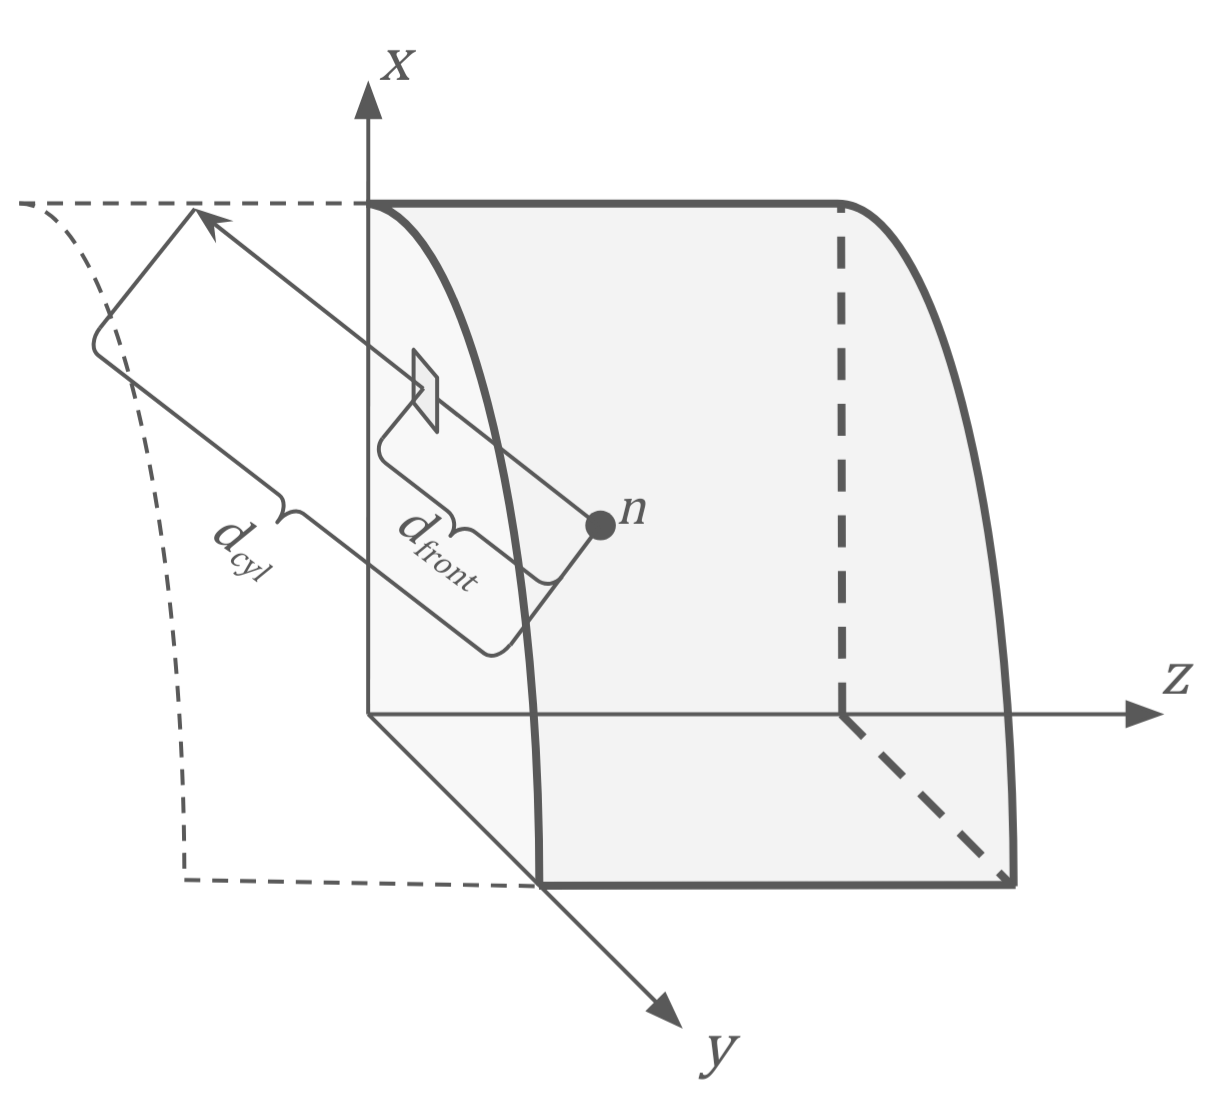
\includegraphics[width=0.75\linewidth]{Figures/ms_face_intersection.png}
    \caption{Example of the face intersection scheme, resulting in $d_{front}$ being selected as the shortest face until the particle exits.}
    \label{fig:ms-face-intersection}
\end{figure}
The $d_{front}$ and $d_{back}$ terms are solved with
\begin{align}
    d_{front} &= \frac{z^k}{\Omega_{z}^{k}} \\
    d_{back} &= \frac{n - z^{k}}{\Omega^{k}_{z}}
\end{align}
while $d_{cyl}$ is is determined as
\begin{equation}
    \label{eq:cyl-intersection-distance}
    d_{cyl} = \frac{\sqrt{b^2 + ac} - b}{a}
\end{equation}
where
\begin{align}
    a &= \left( \Omega_{u}^{k} \right)^2 + \left( \Omega_{v}^{k} \right)^2\\
    b &= x^k \Omega_{u}^{k} + y^k\Omega_{v}^{k} \\
    c &= R^2 - \left( x^k \right)^2 - \left( y^k \right)^2
\end{align}

Once the $d_{front}, d_{back}, \text{ and } d_{cyl}$ distances are determined, the actual path length until escape is
\begin{equation}
    d^k =
    \begin{cases}
        \min{ \left( d_{cyl}, d_{front} \right)},   \qquad &\Omega_{w}^k < 0,\\
        d_{cyl},                                    \qquad &\Omega_{w}^k = 0, \\
        \min{ \left( d_{cyl}, d_{back} \right)},    \qquad &\Omega_{w}^k > 0,\\
    \end{cases}
\end{equation}

Next, a new set of total, capture, and elastic cross sections are sampled at energy $E^k$, which are then used to determine the sampled distance until the next collision,
\begin{equation}
    \label{eq:free-path-sampling}
    s^k = -\frac{1}{\overline{\sigma_{t} }^{k} }  \ln{\left\{
                1 - \zeta \left[ 1 - \exp{\left( \overline{\sigma_{t}}^{k} d^k \right)} \right]
    \right\}}
\end{equation}
where $\zeta$ is a randomly selected value between 0 and 1. This distance term $s^{k}$ is then used to calculate the location of the next scattering event,
\begin{equation}
    \label{eq:sampling-new-location}
    \overrightarrow{x}^{k+1} = \overrightarrow{x}^{k} + \Omega^{k}s^{k}
\end{equation}

\subsubsection{Sampling Energy}
\label{sec:sampling-energy-ms}
The energy in which the neutron leaves the scattering event, i.e., $E^{k+1}$, must be determined. This introduces its own complication, as $E^{k+1}$ is dependent on the mass of the isotope it interacts with, along with its scattering angle. 

First, addressing the mass dependency. This quantity must be sampled according to each isotopes calculated scattering cross section and their given abundances, as
\begin{equation}
    w_{j} = \frac{\delta_j \sigma_{j,sc}^{k} }{\overline{\sigma_{sc}}^{k}}
\end{equation}
This quantity is then used to calculate a cumulative weight, such that
\begin{equation}
    W_j = \sum_{j} w_j
\end{equation}
This defines the window of probability for the scattering event occurring on isotope $j$ as being between $(W_{j-1}, W_{j}]$.
A random number $\zeta$ is sampled between 0 and 1, is used such that
\begin{equation}
    W_{j-1} < \zeta \leq W_{j}
\end{equation}
determines that the neutron will be sampled as scattering off a nucleus with the mass $A_j$.

Next, addressing the angle dependency. The scattering angle is assumed to be isotropic, therefore can scatter with the angle $\phi$, determined as
\begin{equation}
    \phi^k = 2\pi\zeta
\end{equation}
Therefore, the energy $E^{k+1}$ is determined as
\begin{equation}
    E^{k+1} = E^{k} \frac{A_j^{2} + 2A_{j}\cos{\left(\phi^{k}\right) + 1}}{\left( A_{j} + 1 \right)^2}
\end{equation}

\subsubsection{Sampling Direction}
The final component of determining the new parameters of a scattering event include calculating the direction the neutron is traveling, $\overrightarrow{\Omega}^{k+1}$. Similar to \autoref{sec:sampling-energy-ms}, an angle $\theta^k$ must be sampled uniformly in the range $[0,2\pi]$. However $\theta$ must be converted from center of mass scale to lab scale, where
\begin{align}
    \cos{\theta'} &= \frac{1 + A_j \cos{\left( \theta^k \right)}}{\sqrt{1 + \left( A_j\right)^2 + 2A_j\cos{\left(\theta^k \right)}}} \\
    \sin{\theta'} &= \sqrt{1 - \left( \cos{\theta'} \right)^2}
\end{align}
while $\phi=\phi'$.
Determining $\overrightarrow{\Omega}^{k+1}$ from $\overrightarrow{\Omega}^{k}$, $\phi'$, and $\theta'$ proceed according to
\begin{equation}
    \label{eq:direction-calculation-ms}
    \overrightarrow{\Omega}^{k+1} = \begin{bmatrix}
        \Omega^{k+1}_u \\[8pt]
        \Omega^{k+1}_v \\[8pt]
        \Omega^{k+1}_w
    \end{bmatrix}
    = \begin{bmatrix}
        \frac{\Omega_{u}^{k} \Omega_{v}^{k}} { \sqrt{1 - \left(\Omega_{w}^{k}\right)^2 }} &
        \frac{-\Omega_v^k} { \sqrt{1 - \left(\Omega_{w}^{k}\right)^2 }} &
        \Omega_u \\[10pt]
        \frac{\Omega_{v}^{k} \Omega_{w}^{k}} { \sqrt{1 - \left(\Omega_{w}^{k}\right)^2 }} &
        \frac{-\Omega_u^k} { \sqrt{1 - \left(\Omega_{w}^{k}\right)^2 }} &
        \Omega_v \\[10pt]
        \frac{-1} { \sqrt{1 - \left(\Omega_{w}^{k}\right)^2 }} &
        0 &
        \Omega_w
    \end{bmatrix} \times
    \begin{bmatrix}
        \sin{\theta'}\cos{\phi'} \\[8pt]
        \sin{\theta'}\sin{\phi'} \\[8pt]
        \cos{\theta'}
    \end{bmatrix}
\end{equation}
However, in the case where $\left(\Omega_w^k\right)^2 = 1$, \autoref{eq:direction-calculation-ms} cannot be used as it would divide by 0. Instead, the operation
\begin{equation}
        \overrightarrow{\Omega}^{k+1} = \begin{bmatrix}
        \Omega^{k+1}_u \\[8pt]
        \Omega^{k+1}_v \\[8pt]
        \Omega^{k+1}_w
    \end{bmatrix} = \Omega_w^k     \begin{bmatrix}
        \sin{\theta'}\cos{\phi'} \\[8pt]
        \sin{\theta'}\sin{\phi'} \\[8pt]
        \cos{\theta'}
    \end{bmatrix}
\end{equation}
is used instead. Finally, all the components required to sample the subsequent scattering event are obtained: $\overrightarrow{x}^{k+1}$, $\overrightarrow{\Omega}^{k+1}$, and $E^{k+1}$.

\subsubsection{Weighting Neutrons}
\label{sec:killing-neutrons-ms}
A calculation must be made to ensure that sufficient scattering events are being accounted for, but not so many scattering events that it is too computationally expensive, or unrealistic collision events bias the yield in some way.

A weighted importance is used to determine the contribution of a particle to capture yield and when to consider the neutron sufficiently unimportant. This is the same calculation performed by default with MCNP\cite{mcnp}. 

Given the sampled distance $s^{k}$,
\begin{align}
    \label{eq:tot-frac}
    \gamma_{tot}^{k} &=  1 - \exp{ \left(-s^{k} \overline{\sigma_{t}}^{k} \right)} \\
    \label{eq:el-frac}
    \gamma_{sc}^{k} &= \gamma_{tot}^{k} \frac{\overline{\sigma_{sc}}^{k}} {\overline{\sigma_{t}}^{k}} \\
    \label{eq:cap-frac}
    \gamma_{cap}^{k} &= \gamma_{tot}^{k} \frac{\overline{\sigma_{\gamma}}^{k}}{\overline{\sigma_{t}}^{k}}
\end{align}

The neutron weight is determined as a function of the non-captured fraction. Starting out with a weight $w^{0}=1$, the weight of a surviving neutron is the product of each non-captured fraction,
\begin{equation}
    \label{eq:neutron-weight}
    w^{k} = w^{k-1}\gamma_{el}^{k}
\end{equation}

This quantity is used in two ways; first, the factor is used to determine the total number of collisions $K$ that a neutron will experience before it is no longer statistically significant. If the weight ends up less than some cutoff factor, $\varepsilon$, the total number of collisions is reached,
\begin{equation}
    \label{eq:collision-counter}
    K = \min{ \left\{ k : w^{k} \leq \varepsilon \right\}}
\end{equation}

The second purpose of the weighting factor is to determine the total probability of capture after $K$ collisions for a single neutron history. The total probability of a neutron being captured is the sum of all weighted capture events until the collision $K$. The probability that a neutron will be captured at the $k^{th}$ collision is the product of the neutron's surviving weight from the previous collision times the capture interacting fraction $\gamma_{cap}^{k}$. This is given explicitly as
\begin{equation}
    \label{eq:capture-total-prob}
     p = \sum_{k=1}^{K} w^{k-1}\gamma_{cap}^{k}
\end{equation}

\subsection{Calculating The Capture Correction Factor}

The two additional quantities required to calculate the capture correction factor are the energy averaged capture cross-section, $\langle \overline{\sigma_{\gamma}} \rangle$, and energy averaged capture probability, $\langle p \rangle$. These are obtained using the $p$ term from \autoref{eq:capture-total-prob}, and $\overline{\sigma_{\gamma}}^{0}$ from \autoref{eq:average-capture-cross-section}, as
\begin{equation}
    \label{eq:avg-capture-prob}
    \langle p \rangle = \frac{1}{N} \sum_{i=1}^{N} p_{i}
\end{equation}
and
\begin{equation}
    \label{eq:avg-capture-xs}
    \langle \overline{\sigma_{\gamma}} \rangle = \frac{1}{N} \sum_{i=1}^{N} \overline{\sigma_{\gamma}}^{0}_{i}
\end{equation}
where the sum is over $N$ total neutron histories. $p$ and $\overline{\sigma_{\gamma}}$ recieve the $i$ subscript to denote that their quantities refer to the $i^{th}$ neutron history.

These quantities are then used to calculate the capture correction factor,
\begin{equation}
    \label{eq:capture-correction-factor-calc}
    C_{C} = \frac{\langle p \rangle }{\langle \overline{ \sigma_{\gamma} } \rangle n}
\end{equation}
which can then be used in \autoref{eq:correction-thin-sample-approximation} to estimate the energy averaged capture yield $\langle Y \rangle$. 

It should be noted that the average capture cross section $\langle \overline{\sigma_{\gamma}} \rangle$ calculated from \autoref{eq:avg-capture-xs} and $\langle \sigma_{\gamma} \rangle$ are not necessarily the same quantity. The $\langle \overline{\sigma_{\gamma}} \rangle$ is computed via Monte Carlo simulation, while $\langle \sigma_{\gamma} \rangle$ from \autoref{eq:correction-thin-sample-approximation} is calculated analytically. The difference between these two quantities is explored in \autoref{sec:xs-variance-dependence}.
